\section*{Appendix}
\addcontentsline{toc}{section}{Appendix}

\begin{figure*}[htp]
    \centering
    \begin{subfigure}{1\textwidth}
        \centering
        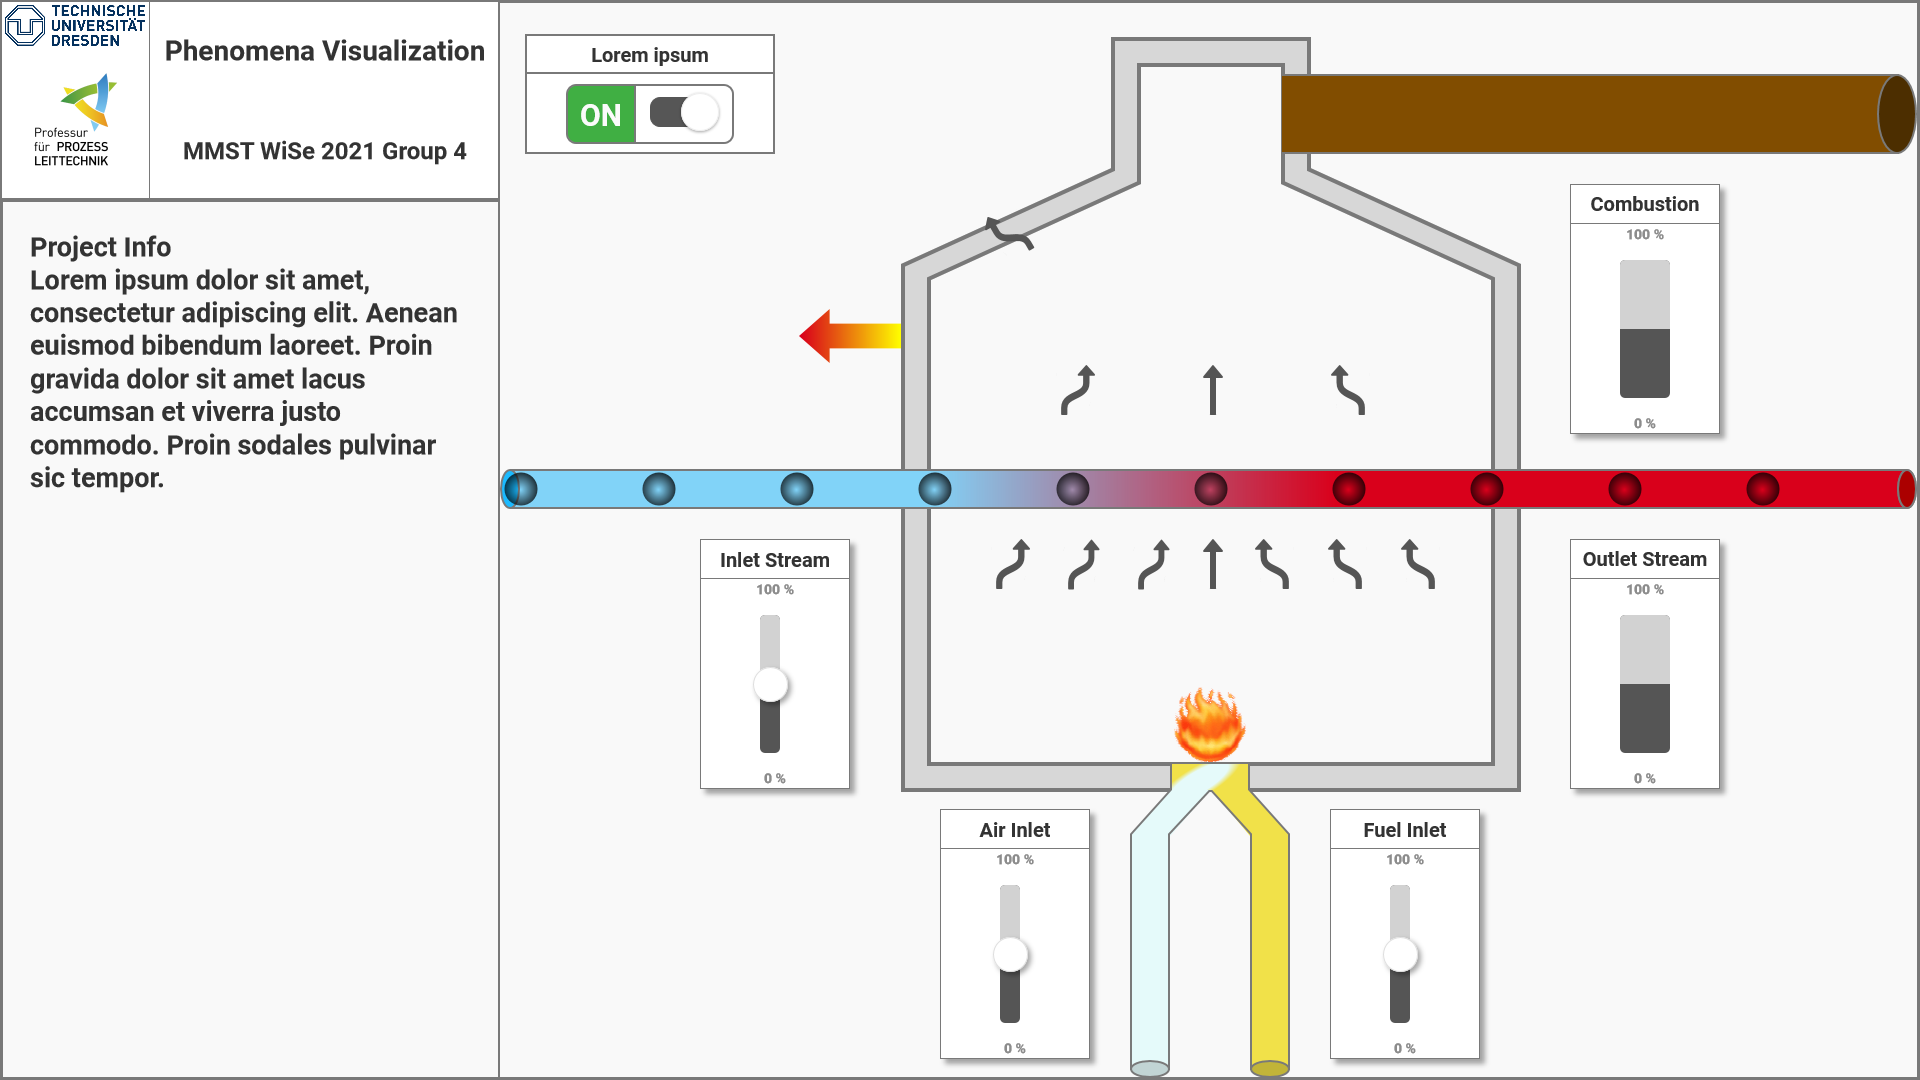
\includegraphics[width=0.9\linewidth]{images/concept/prototype/prototype v1.png}
        \caption{}
    \end{subfigure}
    \\[\baselineskip]
    \begin{subfigure}{1\textwidth}
        \centering
        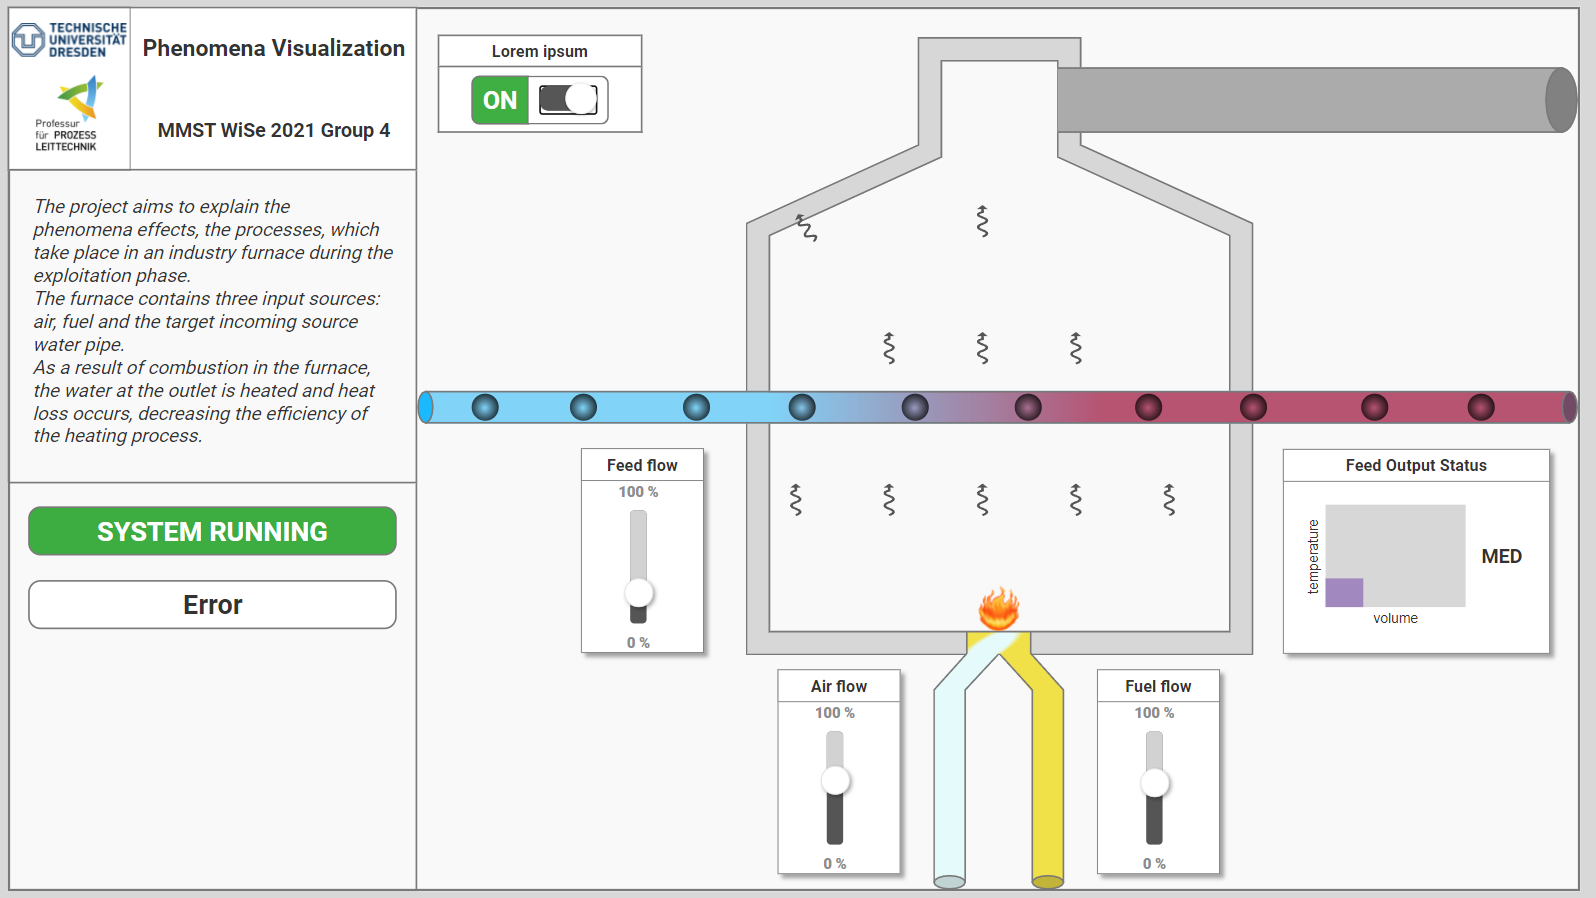
\includegraphics[width=0.9\linewidth]{images/concept/prototype/prototype v2.png}
        \caption{}
    \end{subfigure}
    \caption {(a) early first and (b) second iteration of the axure prototype}
\label{fig:appendix_prototype_early_versions}
\end{figure*}

\begin{figure*}[ht]
    \centering
    \begin{subfigure}{1\textwidth}
        \centering
        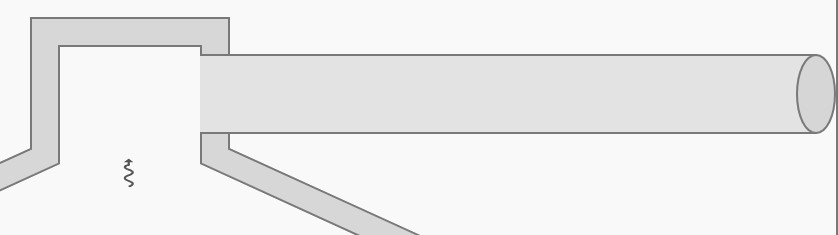
\includegraphics[width=0.6\linewidth]{images/concept/elements/low_combustion_output.jpg}
        \caption{}
    \end{subfigure}
    \\[\baselineskip]
    \begin{subfigure}{1\textwidth}
        \centering
        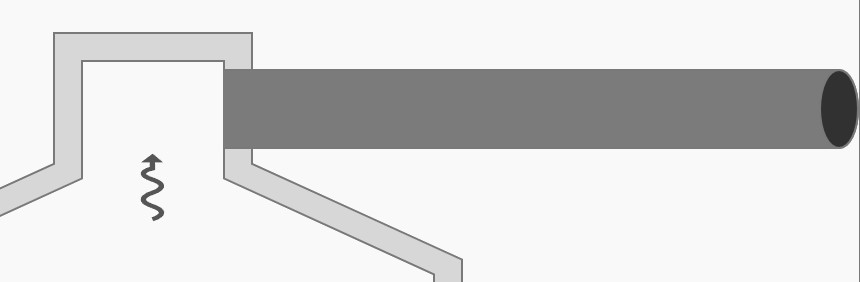
\includegraphics[width=0.6\linewidth]{images/concept/elements/high_combustion_output.jpg}
        \caption{}
    \end{subfigure}
    \caption { (a) small amount of combustion  (b) large amount of combustion}
\label{fig:appendix_combustion_product}
\end{figure*}

 \begin{figure*}[htp]
    \centering
    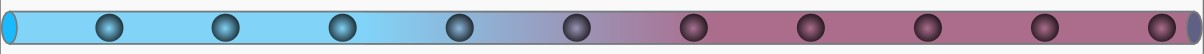
\includegraphics[width=0.9\linewidth]{images/concept/elements/flow_pipe.jpg}
    \caption {feed flow: red = high temperature, light blue = cold temperature}
\label{fig:appendix_flow_pipe}
\end{figure*}

\begin{figure*}[htp]
    \centering
    \begin{subfigure}{0.5\textwidth}
        \centering
        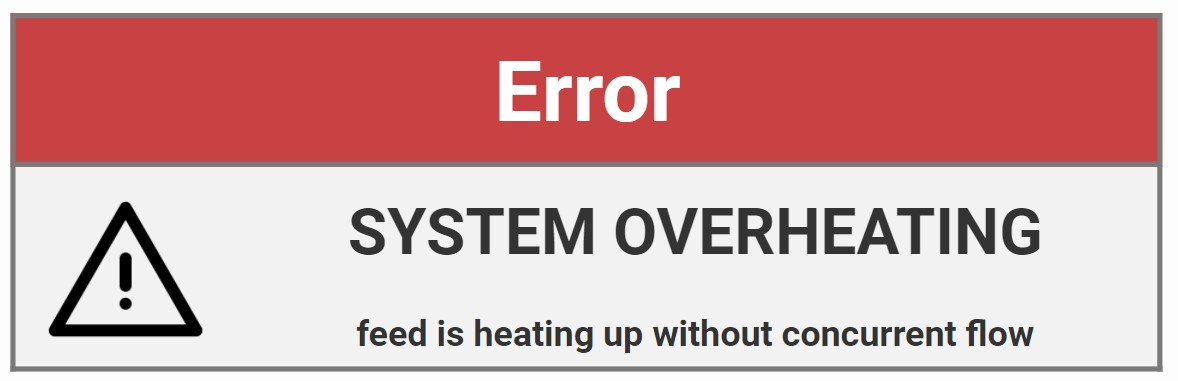
\includegraphics[width=0.9\linewidth]{images/concept/elements/error.jpg}
        \caption{}
    \end{subfigure}%
    \begin{subfigure}{0.5\textwidth}
        \centering
        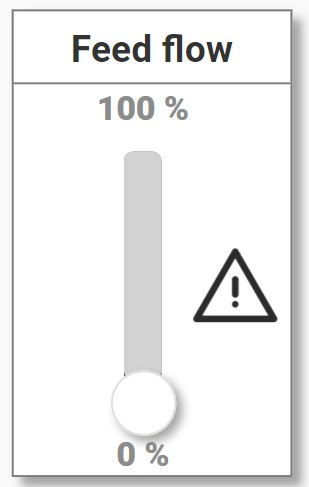
\includegraphics[width=0.4\linewidth]{images/concept/elements/error_feed_flash.jpg}
        \caption{}
    \end{subfigure}
    \caption { (a) side panel error indicator (b) flashing warning sign next to input control}
\label{fig:appendix_error}
\end{figure*}
 
\begin{figure*}[htp]
    \centering
    \begin{subfigure}{0.5\textwidth}
        \centering
        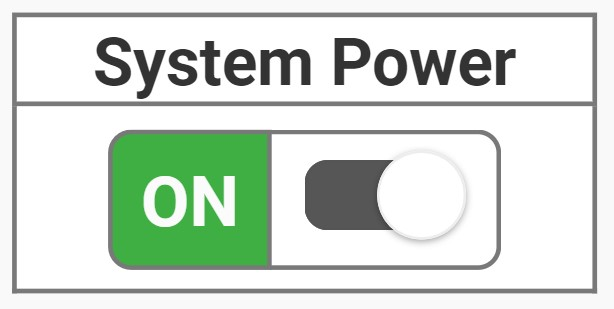
\includegraphics[width=0.6\linewidth]{images/concept/elements/system_power.jpg}
        \caption{}
    \end{subfigure}%
    \begin{subfigure}{0.5\textwidth}
        \centering
        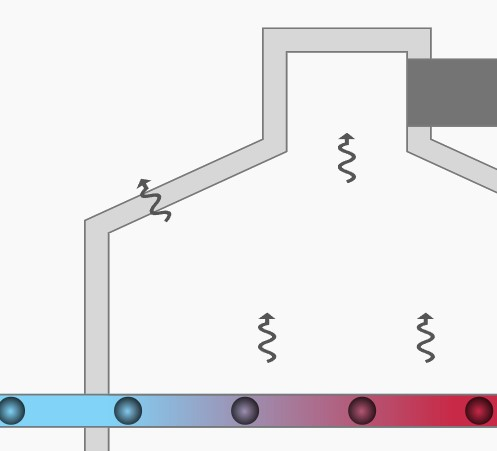
\includegraphics[width=0.7\linewidth]{images/concept/elements/arrow_heatloss.jpg}
        \caption{}
    \end{subfigure}
    \caption { (a) system power switch (b) heatloss shown by corrugated arrows}
\label{fig:appendix_heat_loss_systempower}
\end{figure*}

\begin{figure*}[htp]
    \centering
    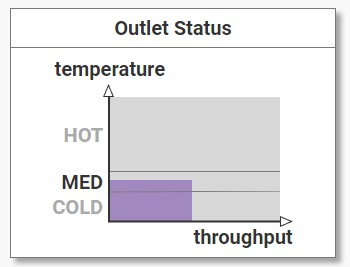
\includegraphics[width=0.5\linewidth]{images/concept/elements/feed_output.jpg}
    \caption {feed output status diagram}
\label{fig:feed_output}
\end{figure*}

\begin{figure*}[htp]
    \centering
    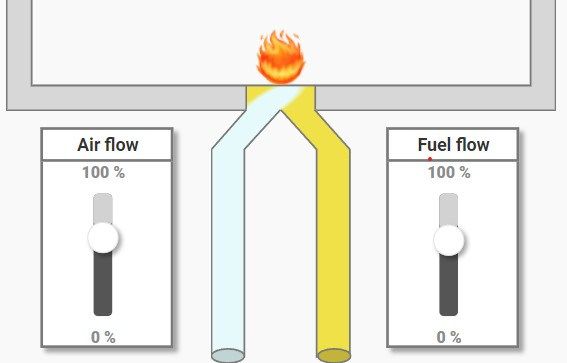
\includegraphics[width=0.7\linewidth]{images/concept/elements/fuel_air_fire.jpg}
    \caption {combustion reaction}
\label{fig:appendix_combustion_reaction}
\end{figure*}




